\chapter{函数类的有限覆盖}
\label{chap:function-class-covers}

设想要预先造好一张函数表，以后无论遇到某一类中的哪个函数，都能从表里查到一行，使它与该函数的最大误差不超过$0.1$。表必须在看到具体函数之前造好，而且只能有有限行。这样的表是否存在，至少需要多少行？

第~\ref{chap:functions-as-vectors}章把函数看作无限维向量，下标是输入$x$，分量是取值$f(x)$。沿着这个类比，一张函数表就是有限个向量，查表就是找最近的向量。在有限维里答案现成：把$\mathbb R^n$中的立方体切成小方块，每个坐标只有有限种取值，方块数是每坐标取值数的$n$次方。可是坐标数趋于无穷时，这个数也趋于无穷。

所以本章的问题可以这样问：一类函数要受到怎样的共同限制，无穷多个坐标才能压缩成有限个有效坐标？答案有两条路线。第一条看取值列，要求相邻坐标互相牵制，只记录有限个位置；第二条看系数列，要求靠后的坐标足够小，只保留前面有限项。

第~\ref{sec:fcover-problem}节把函数表写成覆盖数，并说明只限制范数不够。第~\ref{sec:fcover-arzela-ascoli}节用一致有界与等度连续回答能否覆盖。第~\ref{sec:fcover-construction}节把第一条路线做成可以计数的构造，第~\ref{sec:fcover-finite-representations}节给出第二条路线。这里只研究确定性的计数，怎样构造满足统一逼近前提的有限表示留给第~\ref{chap:function-approximation}章。

\section{有限覆盖问题}
\label{sec:fcover-problem}

函数表问题有三个要素：一类函数，一个衡量误差的距离，一个精度。本节先把它们写成覆盖数，再用有限维的立方体作参照，比较为单个函数找近似与为整类函数造表这两种要求，最后说明只限制范数为什么不够。

\paragraph{函数类与覆盖数}

我们把要讨论的一组函数称为\term{函数类}（function class），记为$\mathcal F$。它总放在某个由函数组成的度量空间$(E,\rho)$中，距离$\rho$就是衡量误差的标准。本章用到的两种距离是
\[
 \lVert f-g\rVert_\infty=\sup_{x\in K}\lvert f(x)-g(x)\rvert,\qquad
 \lVert f-g\rVert_1=\int_0^1\lvert f-g\rvert\,dx .
\]
前者用在紧集$K$上的连续函数空间$C(K)$中，后者用在$L^1[0,1]$中。

函数表的一行就是$E$中的一个函数。表能服务于整类，意思是$\mathcal F$的每个成员都落在某一行的半径$\varepsilon$闭球内。第~\ref{chap:metric-spaces}章把所需的最少行数定义为覆盖数：
\begin{equation}
 N_E(\varepsilon,\mathcal F)=\min\Bigl\{N:\ \exists\,g_1,\ldots,g_N\in E,\
 \mathcal F\subseteq\bigcup_{j=1}^NB[g_j,\varepsilon]\Bigr\},
 \label{eq:fcover-covering-number}
\end{equation}
没有有限覆盖时记为$+\infty$。

覆盖数的对数$\log N_E(\varepsilon,\mathcal F)$称为度量熵。它的含义很具体：给表中的行编号需要$\lceil\log_2N\rceil$个二进制位，例如$N=1024$时需要$10$位。发送这几位，对方查表就能以误差$\varepsilon$复原类中的成员。所以度量熵是在精度$\varepsilon$下识别一个成员所需的信息量。

表中的行可以有两种约定。$N_E(\varepsilon,\mathcal F)$允许行取$E$中任意函数，例如后面用插值造出的折线，它们未必属于$\mathcal F$。$N_{\mathcal F}(\varepsilon,\mathcal F)$要求每一行本身就是类中成员。第~\ref{chap:metric-spaces}章证明了两者只差把精度减半：
\begin{equation}
 N_E(\varepsilon,\mathcal F)\leq N_{\mathcal F}(\varepsilon,\mathcal F)\leq N_E(\varepsilon/2,\mathcal F).
 \label{eq:fcover-center-change}
\end{equation}

右边的不等式后面要反复使用，这里重述它的机制。取一个中心在$E$中的$\varepsilon/2$覆盖，删去与$\mathcal F$不相交的球，在每个余下的球中任选一个成员$g$代替原中心$c$。原来落在该球中的成员$f$到$g$的距离满足
\[
 \rho(f,g)\leq\rho(f,c)+\rho(c,g)\leq\frac\varepsilon2+\frac\varepsilon2=\varepsilon .
\]
所以更换中心不增加行数，只把半径放大一倍。

\paragraph{从立方体到函数}

先看有限维。在$\mathbb R^n$中取最大分量距离
\[
 \lVert a-b\rVert_\infty=\max_k\lvert a_k-b_k\rvert ,
\]
它是一致距离在有限个下标上的版本。半径$\varepsilon$的闭球是边长$2\varepsilon$的小立方体，条件$\lVert a-b\rVert_\infty\leq\varepsilon$就是每个坐标都在$b_k$的$\varepsilon$范围内。

要覆盖立方体$[-M,M]^n$，只需每个坐标各选一组刻度。令$T=\lceil M/\varepsilon\rceil$，取刻度
\[
 c_k=-M+(2k-1)\varepsilon,\qquad k=1,\ldots,T .
\]
区间$[c_k-\varepsilon,c_k+\varepsilon]$首尾相接，覆盖了$[-M,M]$，所以每个坐标都能选到距离不超过$\varepsilon$的刻度。

各坐标的刻度可以任意搭配，全部搭配共$T^n$种，于是
\begin{equation}
 N_{\mathbb R^n}\bigl(\varepsilon,[-M,M]^n\bigr)\leq\Bigl\lceil\frac M\varepsilon\Bigr\rceil^n,\qquad
 \log N_{\mathbb R^n}\leq n\log\Bigl\lceil\frac M\varepsilon\Bigr\rceil .
 \label{eq:fcover-cube}
\end{equation}
度量熵的结构是“坐标个数乘以每个坐标的信息量”，本章后面的上界都是这个结构。

用一个小例子走一遍。下面取$n=3$、$M=1$、$\varepsilon=1/4$，于是$T=4$，刻度为
\[
 -\frac34,\quad -\frac14,\quad \frac14,\quad \frac34 .
\]
式~\eqref{eq:fcover-cube}给出至多$4^3=64$个中心。向量$(0.3,-0.6,0.9)$的最近搭配是$(1/4,-3/4,3/4)$，三个坐标的误差依次是$0.05$、$0.15$、$0.15$，都不超过$1/4$。

函数的情形完全类比。在一致距离下，以$g$为中心、半径$\varepsilon$的闭球由满足
\[
 g(x)-\varepsilon\leq f(x)\leq g(x)+\varepsilon\qquad\text{对所有}\ x
\]
的函数$f$组成。这是图像周围的一条管道，正是小立方体在无穷多个坐标上的样子。

\begin{BookInlineFigure}
  \centering
  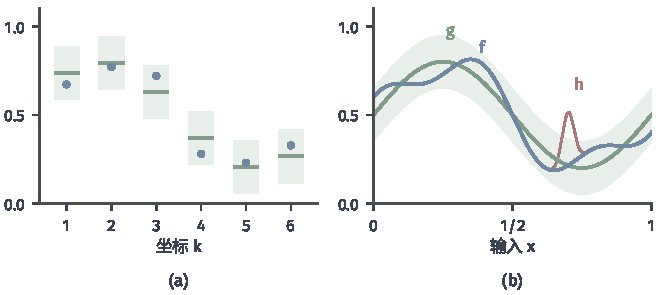
\includegraphics[width=112mm]{figures/04-spaces-measures-and-geometry/03-function-spaces/matplotlib/fcover-cube-tube/figure.pdf}
  \caption{一致距离的闭球。(a)绿色短线是代表$g$的六个坐标，绿色方框是各坐标$\pm\varepsilon$的范围（$\varepsilon=0.15$）；蓝点$f$的六个坐标都在方框内，表示$f$在这个闭球里。(b)同样的$g$与$f$画在全部输入上，方框连成管道。红色的$h$只在一小段上越出管道，一致距离仍把它判在球外。}
  \label{fig:fcover-cube-tube}
\end{BookInlineFigure}

图~\ref{fig:fcover-cube-tube}中，$f$在(a)的每个坐标上都落入方框，(b)中整条曲线留在管道里。一致距离只看最坏的坐标，$h$在别处都贴近$g$，在一小段上越出管道就算不合格。

类比也在这里显出困难。式~\eqref{eq:fcover-cube}的右端随$n$增大而趋于无穷，函数有无穷多个坐标，不能直接套用。真正的问题是：一类函数的无穷多个坐标，能否只用有限多个就决定到精度$\varepsilon$？

\paragraph{挑选近似与统一精度}

先看为单个函数找近似。给定$f\in C[0,1]$和$\varepsilon>0$，$f$在紧区间上一致连续，存在$m$，使$\lvert x-y\rvert\leq1/m$时$\lvert f(x)-f(y)\rvert\leq\varepsilon$。连接点$(j/m,f(j/m))$（$j=0,\ldots,m$）得到折线$g$。

设$x$在第$j$段上，局部位置为$t\in[0,1]$，则$g(x)$是两端值的凸组合，
\[
 f(x)-g(x)=(1-t)\Bigl(f(x)-f\bigl(\tfrac jm\bigr)\Bigr)+t\Bigl(f(x)-f\bigl(\tfrac{j+1}m\bigr)\Bigr).
\]
括号内的两项绝对值都不超过$\varepsilon$，所以$\lvert f(x)-g(x)\rvert\leq\varepsilon$。

这说明每个连续函数都有由$m+1$个数决定的近似，但$m$取决于$f$变化的快慢。为整类函数造表，要求的量词次序不同。两种说法分别是
\[
 \begin{gathered}
 \forall f\in\mathcal F,\ \exists\text{有限描述}\ g_f:\ \rho(f,g_f)\leq\varepsilon,\\
 \exists\text{有限集}\ V\subseteq E,\ \forall f\in\mathcal F,\ \exists v\in V:\ \rho(f,v)\leq\varepsilon .
 \end{gathered}
\]

第一种说法对$C[0,1]$总成立，第二种则要求一份预算服务全类。有限类总能造表，把成员全部列出即可。困难出在无限类上：若所需的节点数$m$随成员无限增大，就没有共同的预算，后面的鼓包正是这样。

\paragraph{距离的选择}

同一类函数在不同距离下可以有不同的答案。向量的情形已经能看出原因：两个$n$维向量只在一个坐标上相差$1$，最大分量差是$1$，平均分量差却只有$1/n$。

取$[0,1]$上的指示函数族$\mathcal F=\{\mathbf 1_{[0,t]}:0\leq t\leq1\}$，每个成员在某一点跳变。在$L^1[0,1]$中，两个成员之差的积分就是图~\ref{fig:fcover-indicator-distances}(b)中矩形的面积：
\[
 \lVert\mathbf 1_{[0,t]}-\mathbf 1_{[0,s]}\rVert_1=\lvert t-s\rvert .
\]
于是覆盖$\mathcal F$等同于用长度$2\varepsilon$的闭区间覆盖参数区间$[0,1]$。

\begin{BookInlineFigure}
  \centering
  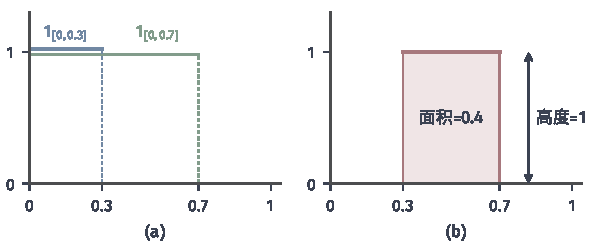
\includegraphics[width=100mm]{figures/04-spaces-measures-and-geometry/03-function-spaces/matplotlib/fcover-indicator-distances/figure.pdf}
  \caption{同一对函数的两种距离。(a)$\mathbf 1_{[0,0.3]}$（蓝）与$\mathbf 1_{[0,0.7]}$（绿）。(b)差的绝对值：$L^1$距离是红色矩形的面积$0.4$，一致距离是矩形的高度$1$。跳变点越靠近，面积越小，高度却始终是$1$。}
  \label{fig:fcover-indicator-distances}
\end{BookInlineFigure}

取$N=\lceil1/(2\varepsilon)\rceil$及$t_j=(2j-1)/(2N)$，每个$t$到最近的$t_j$不超过$1/(2N)\leq\varepsilon$，所以
\[
 N_{\mathcal F}(\varepsilon,\mathcal F)\leq\Bigl\lceil\frac1{2\varepsilon}\Bigr\rceil .
\]
例如$\varepsilon=0.1$时$N=5$，五个中心的跳变点是$0.1,0.3,0.5,0.7,0.9$。成员$\mathbf 1_{[0,0.62]}$对应最近的中心$t=0.7$，误差为$0.08$。

把同一族函数看作$[0,1]$上的有界函数，改用一致距离，情形就变了。$t\neq s$时两个指示函数在$t$与$s$之间相差$1$，所以两两距离都是$1$。半径$\varepsilon<1/2$的闭球若含其中两个，两者距离至多$2\varepsilon<1$，矛盾，因此每个球至多含一个成员。成员有不可数多个，覆盖数为$+\infty$。

积分距离允许误差集中在测度很小的集合上，一致距离不允许，两种答案的分界就在这里。

\paragraph{范数界不能保证有限覆盖}

最直接的约束是给出范数上界，即把$\mathcal F$放进一个闭球。这相当于把每个坐标限制在$[-M,M]$中，在有限维已足够，在无限维却不够。第~\ref{chap:functions-as-vectors}章用Riesz引理证明：任何无限维赋范空间的闭单位球中都有一列单位向量，两两距离至少为$1/2$。

半径$r<1/4$的闭球若含其中两个，两者距离至多$2r<1/2$，矛盾。所以无限维空间的闭单位球不能被半径小于$1/4$的有限个闭球覆盖。按比例缩放，半径$R$的闭球不能被半径小于$R/4$的有限个闭球覆盖。

在$C[0,1]$中可以把这一现象看得很具体。第~\ref{chap:functions-as-vectors}章的鼓包$\varphi_n$在$[\tfrac1{n+1},\tfrac1n]$的中点取$1$，在两端取$0$，区间外恒为$0$。不同鼓包的支撑至多相接于一点，所以$n\neq l$时
\[
 \lVert\varphi_n-\varphi_l\rVert_\infty=1 .
\]
全部$\varphi_n$都在闭单位球内，却没有半径小于$1/2$的有限覆盖。

\begin{BookInlineFigure}
  \centering
  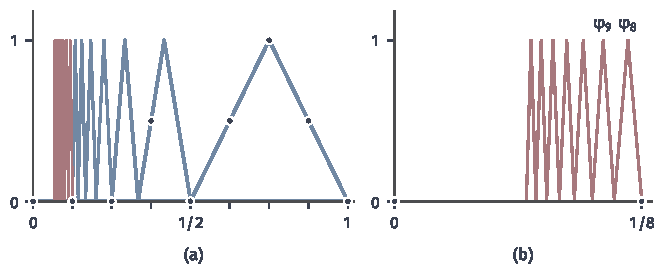
\includegraphics[width=112mm]{figures/04-spaces-measures-and-geometry/03-function-spaces/matplotlib/fcover-tents-on-grid/figure.pdf}
  \caption{固定网格看不见足够窄的鼓包。黑点是节点$j/8$。(a)蓝色为$\varphi_1,\ldots,\varphi_7$，红色为$\varphi_8,\ldots,\varphi_{14}$。(b)把$[0,1/8]$放大：红色鼓包的支撑全在两个节点之间，节点上的值都是$0$。}
  \label{fig:fcover-tents-on-grid}
\end{BookInlineFigure}

失败的原因可以从图~\ref{fig:fcover-tents-on-grid}读出来。固定一组节点$j/m$，当$n\geq m$时，$\varphi_n$的支撑含于$[0,1/m]$，内部没有节点，于是$\varphi_n$在每个节点上都为$0$。这些鼓包与零函数记录相同，一致距离却是$1$。

这也解释了斜率的作用。$\varphi_n$从$0$升到$1$只用了长度$1/(2n(n+1))$的区间，斜率为$2n(n+1)$，随$n$无界。用向量的语言说，每个鼓包占据一段自己的“坐标”，互相之间没有牵制，就像标准单位向量$e_n$。

要补上缺失的条件，有两个方向。第~\ref{sec:fcover-arzela-ascoli}节要求全类共用一个连续性尺度，让相邻坐标互相牵制；第~\ref{sec:fcover-finite-representations}节要求全类都贴近同一个有限维子空间，让靠后的坐标足够小。

\section{Arzelà--Ascoli判据}
\label{sec:fcover-arzela-ascoli}

上一节的帽形函数说明，函数类缺少共同的连续性尺度时，有限个位置上的值无法代表整个函数。本节把这一观察变成判据：在紧度量空间$K$上，连续函数类在一致距离下全有界，当且仅当它一致有界并且等度连续。全节中$C(K)$表示$K$上实值或复值连续函数的全体，距离取$\lVert f-g\rVert_\infty$；两种取值情形的论证相同，只在量化取值时分别处理实轴上的区间与复平面上的正方形。

\paragraph{一致有界与等度连续}

覆盖要求有限个代表照顾到每个成员，因此类中函数至少要共同受到两方面的约束：取值不能任意大，变化不能任意快。第一个约束是幅度上的。

\begin{definition}[一致有界]
\label{def:fcover-uniformly-bounded}
设$K$是集合，$\mathcal F$是$K$上一族实值或复值函数。若存在常数$M$，使$\lvert f(x)\rvert\leq M$对所有$f\in\mathcal F$和所有$x\in K$成立，就称$\mathcal F$\term{一致有界}（uniformly bounded）。
\end{definition}

对$\mathcal F\subseteq C(K)$，一致有界就是$\sup_{f\in\mathcal F}\lVert f\rVert_\infty<\infty$，即$\mathcal F$含于一个一致范数球中。上一节的帽形函数说明，仅有这一条还不够。

第二个约束是变化上的，它就是第~\ref{chap:metric-space-maps}章的等度连续性：对每个$x\in K$和$\varepsilon>0$，有一个对全族都有效的半径$\delta$，使$d(x,y)<\delta$时$\lvert f(x)-f(y)\rvert<\varepsilon$对所有$f\in\mathcal F$成立。那里还证明了，定义域紧时这个半径可以进一步取得与$x$无关。下面使用的正是这一统一形式：对每个$\varepsilon>0$，存在$\delta>0$，使
\begin{equation}
d(x,y)<\delta\ \Longrightarrow\ \lvert f(x)-f(y)\rvert<\varepsilon\qquad\text{对所有}\ f\in\mathcal F\ \text{及}\ x,y\in K.
\label{eq:fcover-uniform-equicontinuity}
\end{equation}

最常见的等度连续族共用一个Lipschitz常数。若每个$f\in\mathcal F$都满足$\lvert f(x)-f(y)\rvert\leq L\,d(x,y)$，取$\delta=\varepsilon/L$即可满足式\eqref{eq:fcover-uniform-equicontinuity}。反过来，上一节的帽形函数$\varphi_k$不等度连续：对任意$\delta>0$，取$k$使$r_k<\delta$，点$x=c_k$与$y=c_k+r_k$相距$r_k<\delta$，却有$\lvert\varphi_k(x)-\varphi_k(y)\rvert=1$。$[0,1]$上的$x^n$也是这样，第~\ref{chap:functions-as-vectors}章已看到它们一致有界却没有一致收敛的子列。

\paragraph{判据与证明}

两个约束合起来恰好刻画全有界性。在陈述之前回忆两件事：$C(K)$在一致距离下完备（第~\ref{chap:normed-spaces}章）；在完备度量空间中，子集相对紧（闭包紧）当且仅当它全有界（第~\ref{chap:metric-spaces}章）。

\begin{theorem}[Arzelà--Ascoli判据]
\label{thm:fcover-arzela-ascoli}
设$(K,d)$是非空紧度量空间，$\mathcal F\subseteq C(K)$，距离取一致距离。则下列三条等价：
\begin{enumerate}
\item $\mathcal F$一致有界且等度连续；
\item $\mathcal F$全有界，即对每个$\varepsilon>0$都有$N_{\mathcal F}(\varepsilon,\mathcal F)<\infty$；
\item $\mathcal F$在$C(K)$中相对紧。
\end{enumerate}
进一步，$\mathcal F$在$C(K)$中紧，当且仅当它满足上述条件并且是$C(K)$的闭子集。
\end{theorem}

证明的核心是有限化：等度连续允许只在有限个位置上观察函数，一致有界允许把这些位置上的值归入有限个小块，于是整类函数只留下有限种“记录”。

\begin{proof}
由1推出2。设$\lvert f\rvert\leq M$对所有$f\in\mathcal F$成立，给定$\varepsilon>0$。由式\eqref{eq:fcover-uniform-equicontinuity}取$\delta>0$，使$d(x,y)<\delta$时$\lvert f(x)-f(y)\rvert<\varepsilon/4$对所有$f$成立。紧空间全有界，所以有有限个点$x_1,\ldots,x_p\in K$，使每个$x\in K$都满足某个$d(x,x_i)<\delta$。

再把取值集合$\{z:\lvert z\rvert\leq M\}$分成有限个直径不超过$\varepsilon/4$的小块：实值时用长度不超过$\varepsilon/4$的小区间，复值时用边长不超过$\varepsilon/(4\sqrt2)$的小正方形，并约定各块互不相交。对每个$f\in\mathcal F$，记下$f(x_1),\ldots,f(x_p)$分别落在哪一块，这一串块编号称为$f$的记录。块数有限、位置数有限，所以记录只有有限种。

对每一种实际出现的记录，从$\mathcal F$中任取一个具有该记录的成员作为代表。若$f$与代表$g$记录相同，则$\lvert f(x_i)-g(x_i)\rvert\leq\varepsilon/4$对每个$i$成立。对任意$x\in K$，取$x_i$使$d(x,x_i)<\delta$，由三角不等式，
\[
\lvert f(x)-g(x)\rvert\leq\lvert f(x)-f(x_i)\rvert+\lvert f(x_i)-g(x_i)\rvert+\lvert g(x_i)-g(x)\rvert<\frac{3\varepsilon}{4}.
\]
所以有限个代表构成中心在$\mathcal F$中的$\varepsilon$覆盖，$N_{\mathcal F}(\varepsilon,\mathcal F)<\infty$。

由2推出1。取一个有限的$1$覆盖$f_1,\ldots,f_N\in\mathcal F$，每个$f$都满足某个$\lVert f-f_j\rVert_\infty\leq1$，故$\lVert f\rVert_\infty\leq\max_j\lVert f_j\rVert_\infty+1$，这就是一致有界。为证等度连续，给定$\varepsilon>0$，取有限的$\varepsilon/3$覆盖$f_1,\ldots,f_N\in\mathcal F$。紧集上的连续函数一致连续（第~\ref{chap:metric-space-maps}章），有限个函数可以共用一个$\delta$，使$d(x,y)<\delta$时$\lvert f_j(x)-f_j(y)\rvert<\varepsilon/3$对每个$j$成立。对任意$f$，选$f_j$使$\lVert f-f_j\rVert_\infty\leq\varepsilon/3$，则
\[
\lvert f(x)-f(y)\rvert\leq\lvert f(x)-f_j(x)\rvert+\lvert f_j(x)-f_j(y)\rvert+\lvert f_j(y)-f(y)\rvert<\varepsilon .
\]

2与3等价。$C(K)$完备，由前面回忆的相对紧判据即得。

最后，紧集是闭集；反过来，若$\mathcal F$相对紧且闭，则$\mathcal F$等于它的闭包，因而紧。
\end{proof}

两个方向的证明各说明了一件事。充分性的构造是可以计数的：位置数$p$由定义域在尺度$\delta$下的覆盖数决定，块数由幅度$M$与精度决定，记录种数至多是块数的$p$次方。第~\ref{sec:fcover-construction}节将在$[0,1]^d$上把这个计数写成显式公式。必要性则说明有限覆盖必然带来共同的连续性尺度，因为有限个函数总能共用一个$\delta$，一致距离再把这个$\delta$传给整个类。

\paragraph{相对紧性与闭性}

定理的最后一句把紧性分成两部分：一致有界与等度连续保证闭包紧，函数类自身紧还需要闭性。这两部分确实不同，下面各举一例。

先看闭的情形。设$L,M>0$，令$\mathcal F_{L,M}$为$K$上满足$\lvert f\rvert\leq M$且$\lvert f(x)-f(y)\rvert\leq L\,d(x,y)$的全体函数。它一致有界且等度连续。若$f_n\in\mathcal F_{L,M}$一致收敛到$f$，则对每一对$x,y$，不等式$\lvert f_n(x)\rvert\leq M$与$\lvert f_n(x)-f_n(y)\rvert\leq L\,d(x,y)$在$n\to\infty$时保持，所以$f\in\mathcal F_{L,M}$。因此$\mathcal F_{L,M}$闭，从而在$C(K)$中紧。

再看不闭的情形。在$[0,1]$上取满足$\lvert f\rvert\leq1$、$\lvert f'\rvert\leq1$的全体连续可微函数。由中值定理，它们共用Lipschitz常数$1$，所以这一类相对紧。但它不闭：令$g_n(x)=\sqrt{(x-1/2)^2+1/n^2}$（$n\geq2$），则$g_n$连续可微，$\lvert g_n'(x)\rvert=\lvert x-1/2\rvert/g_n(x)<1$，且$g_n\leq\sqrt{1/4+1/4}<1$。又
\[
0\leq g_n(x)-\Bigl\lvert x-\frac12\Bigr\rvert=\frac{1/n^2}{g_n(x)+\lvert x-1/2\rvert}\leq\frac1n,
\]
所以$g_n$一致收敛到在$1/2$处不可导的$\lvert x-1/2\rvert$。这一类的闭包是紧的，它自身却不紧，极限跑到了类外。

\paragraph{定义域紧性的作用}

判据中的紧定义域同样不能省略。证明充分性时，我们用有限个点$x_1,\ldots,x_p$控制了整个定义域，这一步依赖$K$的全有界性。若定义域是$\mathbb R$，即使函数类一致有界且共用一个Lipschitz常数，也可能没有有限覆盖。

取$\varphi(x)=\max\{0,1-\lvert x\rvert\}$及平移族$\varphi_n(x)=\varphi(x-3n)$，$n\in\mathbb Z$。全族满足$0\leq\varphi_n\leq1$，Lipschitz常数都是$1$。但$\varphi_n$与$\varphi_m$（$n\neq m$）的支撑相距至少$1$，在$3n$处两者相差$1$，所以$\sup_x\lvert\varphi_n(x)-\varphi_m(x)\rvert=1$。半径小于$1/2$的球至多含一个成员，覆盖数为$+\infty$。函数之间的差异跑向了无穷远，有限个位置看不到它。

\section{有限覆盖的构造}
\label{sec:fcover-construction}

Arzelà--Ascoli判据只断言有限覆盖存在。要知道需要多少个代表，就要把证明中的“有限位置、有限取值”换成可以计数的具体构造。本节固定一类具体对象：$[0,1]^d$上满足
\[
\lvert f(x)\rvert\leq M,\qquad \lvert f(x)-f(y)\rvert\leq L\lVert x-y\rVert_\infty\qquad(x,y\in[0,1]^d)
\]
的实值函数全体，记为$\mathcal F^d_{L,M}$，其中$L,M>0$，$\lVert x\rVert_\infty=\max_i\lvert x_i\rvert$。误差用$C([0,1]^d)$上的一致距离衡量。若题设给的是欧氏距离下的Lipschitz常数$L'$，由$\lVert x\rVert_2\leq\sqrt d\lVert x\rVert_\infty$可取$L=\sqrt d\,L'$。

上一节已经说明这一类在一致距离下紧。构造的思路是把总误差$\varepsilon$拆成两份预算：一份给位置离散化，只在网格点上记录函数时，网格点之间的变化要受控；另一份给取值量化，网格点上的实数要换成有限个刻度之一。Lipschitz界控制前者，幅值界决定后者需要多少刻度。

\subsection{网格误差与取值误差}
\label{sec:fcover-grid-and-quantization}

\paragraph{网格与多线性插值}

取正整数$m$，网格$G_m$由坐标都属于$\{0,1/m,\ldots,1\}$的点组成，共$(m+1)^d$个节点。网格把$[0,1]^d$分成$m^d$个边长为$1/m$的小立方体单元。只知道函数在节点上的值时，需要一种方法把这些值填满每个单元，并且填出的函数仍然连续。一维时自然的做法是连折线，高维时把折线逐坐标推广。

设$a$是定义在$G_m$上的实值函数。对单元$Q=\prod_{i=1}^d[j_i/m,(j_i+1)/m]$中的点$x$，记局部坐标$t_i=mx_i-j_i\in[0,1]$。\term{多线性插值}（multilinear interpolation）定义为
\begin{equation}
(Ia)(x)=\sum_{e\in\{0,1\}^d}a\Bigl(\frac{j+e}{m}\Bigr)\prod_{i=1}^d w_{e_i}(t_i),\qquad w_1(t)=t,\quad w_0(t)=1-t .
\label{eq:fcover-multilinear}
\end{equation}
这里$e$遍历单元的$2^d$个顶点，顶点$(j+e)/m$的权重是各坐标方向上一维折线权重的乘积。$d=1$时，式\eqref{eq:fcover-multilinear}就是$(1-t)a(j/m)+t\,a((j+1)/m)$，即连接相邻节点值的折线。

这一定义有三条性质。第一，权重非负，且$\sum_e\prod_iw_{e_i}(t_i)=\prod_i\bigl((1-t_i)+t_i\bigr)=1$，所以$(Ia)(x)$是所在单元顶点值的凸组合。第二，在顶点处只有一个权重等于$1$，所以$Ia$在节点上取值$a$。第三，在两个单元的公共面上，例如$t_i=1$时，所有$e_i=0$的顶点权重为零，只剩公共面上的顶点；邻接单元中同一点的局部坐标为$t_i=0$，留下的也正是这些顶点，权重相同。因此两侧公式在公共面上一致，$Ia$是$[0,1]^d$上的连续函数。

\paragraph{两类误差的分别控制}

给定$f\in\mathcal F^d_{L,M}$，把它在节点上的值记为$f|_{G_m}$。再取刻度间距$2\eta$，令$K=\lceil M/\eta\rceil$，刻度为$c_k=-M+(2k-1)\eta$（$k=1,\ldots,K$）。相邻刻度相距$2\eta$，首末刻度满足$c_1=-M+\eta$、$c_K\geq M-\eta$，所以$[-M,M]$中每个数到最近刻度的距离不超过$\eta$。把每个节点值换成最近的刻度（等距时取较小者），得到量化值$q_f$。这一步称为\term{量化}（quantization），它让节点值只剩$K$种可能。

用$Iq_f$作$f$的代表，由三角不等式，
\[
\lVert f-Iq_f\rVert_\infty\leq\underbrace{\lVert f-I(f|_{G_m})\rVert_\infty}_{\text{网格误差}}+\underbrace{\lVert I(f|_{G_m})-Iq_f\rVert_\infty}_{\text{取值误差}} .
\]
两项分别只与一种预算有关。网格误差：设$x$属于某个单元，该单元的每个顶点$v$都满足$\lVert x-v\rVert_\infty\leq1/m$。由凸组合性质，
\[
\lvert f(x)-I(f|_{G_m})(x)\rvert=\Bigl\lvert\sum_v w_v\bigl(f(x)-f(v)\bigr)\Bigr\rvert\leq\sum_vw_v\,\frac Lm=\frac Lm ,
\]
其中$w_v$是式\eqref{eq:fcover-multilinear}中顶点$v$的权重。取值误差：$I$对节点值是线性的，凸组合给出$\lvert(Ia)(x)-(Ib)(x)\rvert\leq\max_{v\in G_m}\lvert a(v)-b(v)\rvert$，而$f|_{G_m}$与$q_f$在每个节点相差不超过$\eta$，所以这一项不超过$\eta$。

\begin{theorem}[Lipschitz类的网格覆盖]
\label{thm:fcover-grid-cover}
对正整数$m$与$\eta>0$，记$K=\lceil M/\eta\rceil$，则
\[
N_{C([0,1]^d)}\Bigl(\frac Lm+\eta,\ \mathcal F^d_{L,M}\Bigr)\leq K^{(m+1)^d}.
\]
特别地，取$m=\lceil2L/\varepsilon\rceil$、$\eta=\varepsilon/2$，得
\begin{equation}
N_{C([0,1]^d)}(\varepsilon,\mathcal F^d_{L,M})\leq\Bigl\lceil\frac{2M}{\varepsilon}\Bigr\rceil^{(\lceil2L/\varepsilon\rceil+1)^d}.
\label{eq:fcover-grid-bound}
\end{equation}
\end{theorem}

\begin{proof}
所有可能的量化节点值$q:G_m\to\{c_1,\ldots,c_K\}$至多有$K^{(m+1)^d}$种，相应的函数$Iq$组成一个有限集。上面的两类误差估计说明，每个$f\in\mathcal F^d_{L,M}$到$Iq_f$的一致距离不超过$L/m+\eta$。代入$m=\lceil2L/\varepsilon\rceil$与$\eta=\varepsilon/2$，有$L/m\leq\varepsilon/2$，总误差不超过$\varepsilon$。
\end{proof}

\paragraph{代表取在类外}

定理中的代表$Iq$取在环境空间$C([0,1]^d)$中，它们未必属于$\mathcal F^d_{L,M}$：量化可能把相邻节点值推向相反方向，使插值函数的斜率超过$L$。例如$d=1$、$L=0.01$、$M=1$、$\varepsilon=0.1$时，$m=1$、$\eta=0.05$，刻度为$\pm0.05,\pm0.15,\ldots$。函数$f(x)=0.01(x-1/2)$在$0$和$1$处的值$\mp0.005$分别量化为$-0.05$和$0.05$，插值折线的斜率为$0.1$，不在类中。

若要求代表本身属于函数类，可以用式\eqref{eq:fcover-center-change}调整半径：$N_{\mathcal F}(\varepsilon,\mathcal F)\leq N_{C([0,1]^d)}(\varepsilon/2,\mathcal F)$，即以$\varepsilon/2$运行上面的构造，再用类中成员替换中心。代价只是把精度参数减半。

以$d=1$、$L=M=1$、$\varepsilon=0.1$为例。此时$m=20$，共$21$个节点，$\eta=0.05$，刻度数$K=20$，式\eqref{eq:fcover-grid-bound}给出$N_{C[0,1]}(0.1,\mathcal F^1_{1,1})\leq20^{21}$，度量熵（自然对数）不超过$21\ln20\approx62.9$。若要求中心在类内，改用$\varepsilon/2=0.05$，得$m=40$、$K=40$，上界为$40^{41}$，度量熵不超过$41\ln40\approx151.2$。

\subsection{覆盖数的维数依赖}
\label{sec:fcover-dimension-dependence}

\paragraph{上界中的四个量}

对式\eqref{eq:fcover-grid-bound}取对数，
\begin{equation}
\log N_{C([0,1]^d)}(\varepsilon,\mathcal F^d_{L,M})\leq\Bigl(\Bigl\lceil\frac{2L}{\varepsilon}\Bigr\rceil+1\Bigr)^d\log\Bigl\lceil\frac{2M}{\varepsilon}\Bigr\rceil .
\label{eq:fcover-entropy-bound}
\end{equation}
右边第一个因子是节点数，第二个因子是每个节点上一个刻度编号的信息量。维数$d$出现在节点数的指数上：精度减半，节点数约乘以$2^d$。Lipschitz界$L$通过网格的细度进入节点数，因而按$(L/\varepsilon)^d$起作用；幅值界$M$只决定刻度数，只在对数中出现。

把这一结果与有限维参数族比较，可以看出Lipschitz类的“大小”。若函数由$p$个有界参数线性决定，度量熵大致按$p\log(1/\varepsilon)$增长，参数个数是固定的（第~\ref{sec:fcover-finite-representations}节）。式\eqref{eq:fcover-entropy-bound}中起参数个数作用的节点数却随精度增长，精度越高需要记录的位置越多，这反映了Lipschitz类是无限维的。下表列出$L=M=1$、$\varepsilon=0.1$时上界随维数的变化。

\begin{table}[!htb]
  \centering
  \caption{$L=M=1$、$\varepsilon=0.1$时式\eqref{eq:fcover-entropy-bound}的各项。每个节点的刻度数都是$20$，节点数按$21^d$增长，度量熵上界（自然对数）随之按同一比例增长。}
  \label{tab:fcover-dimension}
  \begin{tabular}{@{}cccc@{}}
    \toprule
    $d$ & 节点数$21^d$ & 每节点刻度数 & 度量熵上界\\
    \midrule
    $1$ & $21$ & $20$ & $62.9$\\
    $2$ & $441$ & $20$ & $1321.1$\\
    $3$ & $9261$ & $20$ & $27743.5$\\
    \bottomrule
  \end{tabular}
\end{table}

\paragraph{利用相邻位置的约束}

式\eqref{eq:fcover-entropy-bound}是可以逐步核验的上界，却不是最优的。它把各节点上的刻度当作互相独立的选择，而Lipschitz条件实际上约束了相邻节点：相距$1/m$的两个节点，函数值相差不超过$L/m$。利用这一约束，可以去掉主项中的对数因子。

把网格节点排成一列$v_0,v_1,\ldots,v_{n-1}$（$n=(m+1)^d$），使相邻两项只在一个坐标上相差$1/m$。这样的“蛇形”次序存在：$d=1$时按$0,1/m,\ldots,1$排列；若$d-1$维网格已排好，就逐层处理最后一个坐标，每层沿$d-1$维次序走完，相邻层交替使用正向与反向，于是一层的末点与下一层的首点只在最后一个坐标上相差$1/m$。

仍取$m=\lceil2L/\varepsilon\rceil$、$\eta=\varepsilon/2$，则$L/m\leq\eta$。对$f\in\mathcal F^d_{L,M}$，相邻量化值满足
\[
\lvert q_f(v_{r+1})-q_f(v_r)\rvert\leq\eta+\frac Lm+\eta\leq3\eta .
\]
刻度差是$2\eta$的整数倍，所以它只能是$-2\eta$、$0$或$2\eta$。量化值序列因而由首项（$K$种）和后面$n-1$个“降、平、升”的选择决定，至多有$K\cdot3^{n-1}$种，于是
\begin{equation}
\log N_{C([0,1]^d)}(\varepsilon,\mathcal F^d_{L,M})\leq\log\Bigl\lceil\frac{2M}{\varepsilon}\Bigr\rceil+\Bigl(\Bigl(\Bigl\lceil\frac{2L}{\varepsilon}\Bigr\rceil+1\Bigr)^d-1\Bigr)\log3 .
\label{eq:fcover-entropy-improved}
\end{equation}
前面$d=1$、$L=M=1$、$\varepsilon=0.1$的例子中，上界从$62.9$降到$\ln20+20\ln3\approx25.0$。

\paragraph{打包下界}

上界改进到哪一步才算够，要靠下界判断。下界来自第~\ref{chap:metric-spaces}章的打包思路：若类中有一组成员两两距离大于$2\varepsilon$，任何半径$\varepsilon$的闭球至多含其中一个，覆盖数就不小于这组成员的个数。下面在每个小单元里放一个可正可负的隆起。

设$L\geq6\varepsilon$且$\varepsilon\leq M/3$。令$k=\lfloor L/(3\varepsilon)\rfloor$、$h=1/k$，把$[0,1]^d$分成$k^d$个边长$h$的单元，单元$Q$的中心记为$c_Q$。在每个单元上取隆起$\varphi_Q(x)=\max\{0,Lh/2-L\lVert x-c_Q\rVert_\infty\}$，它支撑在$Q$上，在$Q$的边界上为零，高度为$Lh/2$。对每个符号选择$s\in\{-1,1\}^{k^d}$，令$g_s=\sum_Qs_Q\varphi_Q$。

先核对$g_s\in\mathcal F^d_{L,M}$。由$k\geq L/(3\varepsilon)-1\geq L/(6\varepsilon)$得高度$Lh/2=L/(2k)\leq3\varepsilon\leq M$。每个$\varphi_Q$关于$\lVert\cdot\rVert_\infty$的Lipschitz常数为$L$；对任意$x,y$，线段$[x,y]$与每个单元的交是一段子线段，在每段上$g_s$等于单个$\pm\varphi_Q$，而$g_s$连续，所以沿线段逐段累加得$\lvert g_s(x)-g_s(y)\rvert\leq L\lVert x-y\rVert_\infty$。

再看距离。两个不同的符号选择$s\neq s'$在某个单元$Q$上不同，在中心$c_Q$处$\lvert g_s-g_{s'}\rvert=2\cdot Lh/2=Lh$。由$k\leq L/(3\varepsilon)$得$Lh=L/k\geq3\varepsilon>2\varepsilon$。所以这$2^{k^d}$个函数两两距离大于$2\varepsilon$，即使中心可取在整个$C([0,1]^d)$中，也有
\[
\log N_{C([0,1]^d)}(\varepsilon,\mathcal F^d_{L,M})\geq k^d\log2\geq\Bigl(\frac{L}{6\varepsilon}\Bigr)^d\log2 .
\]

\paragraph{上界与最优阶}

把下界与式\eqref{eq:fcover-entropy-improved}放在一起，固定$L,M,d$而令$\varepsilon\to0$时，度量熵夹在$(L/\varepsilon)^d$的两个常数倍之间，这就是它的增长阶；幅值$M$只影响低阶的对数项。Kolmogorov与Tikhomirov系统研究了这类函数类的度量熵，给出了更精确的常数与更多正则性类的结果\scite{kolmogorov1959epsilon}。

本节的经验是：直接的网格量化总能给出可以逐项核验的上界，参数选择与误差来源都一目了然；但要判断上界是否已达最优阶，还需要利用不同位置之间的约束改进编码，并构造相应的打包集给出下界。

\section{由有限表示构造覆盖}
\label{sec:fcover-finite-representations}

第~\ref{chap:functions-as-vectors}章说过，一个函数有两种“一列数”：取值列，下标是输入；系数列，下标是基函数的编号。上一节截取的是取值列，节点数随精度增长。本节换成系数列：若整类函数都能用同一组有限个基函数统一逼近，只是各自的系数不同，靠后的系数就可以整体舍去，覆盖问题分成两步，先把每个成员换成有限维子空间中的近似，再覆盖这些近似组成的有限维有界集。

\paragraph{统一逼近与有限维球}

设$(E,\lVert\cdot\rVert)$是实赋范函数空间，$V\subseteq E$是$n$维子空间。第~\ref{chap:metric-spaces}章证明了：在$n$维实赋范空间中，半径$R$的闭球可以被至多$(1+2R/\varepsilon_1)^n$个半径$\varepsilon_1$的闭球覆盖，中心取在该空间内。这就是立方体计数式~\eqref{eq:fcover-cube}的一般形式。把它用于$V$及$E$限制在$V$上的范数，就得到下面的结论。

\begin{theorem}[有限维统一逼近给出覆盖]
\label{thm:fcover-finite-dimensional}
设$\mathcal F\subseteq E$，$\varepsilon_0\geq0$，$R>0$。若对每个$f\in\mathcal F$都存在$g_f\in V$，使
\begin{equation}
 \lVert f-g_f\rVert\leq\varepsilon_0,\qquad\lVert g_f\rVert\leq R,
 \label{eq:fcover-uniform-approximation}
\end{equation}
则对每个$\varepsilon_1>0$，
\begin{equation}
 N_E(\varepsilon_0+\varepsilon_1,\mathcal F)\leq\Bigl(1+\frac{2R}{\varepsilon_1}\Bigr)^n .
 \label{eq:fcover-finite-dimensional}
\end{equation}
\end{theorem}

\begin{proof}
若$\varepsilon_1>R$，以零函数为中心、半径$\varepsilon_1$的闭球已含$V$中半径$R$的闭球，一个中心足够。下设$\varepsilon_1\leq R$，取$V$中半径$R$闭球的一个$\varepsilon_1$覆盖，中心$v_1,\ldots,v_N\in V$，$N\leq(1+2R/\varepsilon_1)^n$。

对$f\in\mathcal F$，$g_f$落在这个闭球中，所以有某个$v_j$满足$\lVert g_f-v_j\rVert\leq\varepsilon_1$。由三角不等式，
\[
 \lVert f-v_j\rVert\leq\lVert f-g_f\rVert+\lVert g_f-v_j\rVert\leq\varepsilon_0+\varepsilon_1 .
\]
所以中心$v_1,\ldots,v_N$构成$\mathcal F$的$(\varepsilon_0+\varepsilon_1)$覆盖。
\end{proof}

\begin{BookInlineFigure}
  \centering
  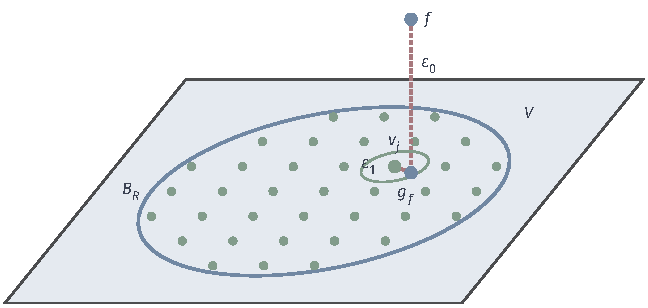
\includegraphics[width=109.7mm]{figures/04-spaces-measures-and-geometry/03-function-spaces/tikz/fcover-two-step/figure.pdf}
  \caption{两步覆盖的几何图景。平面是$n$维子空间$V$，蓝色椭圆是其中半径$R$的闭球，绿点是该球的$\varepsilon_1$网。$f$在$V$之外，先走到$V$中的近似$g_f$（红色虚线，长度不超过$\varepsilon_0$），再走到最近的网点$v_j$（红色实线，长度不超过$\varepsilon_1$）。}
  \label{fig:fcover-two-step}
\end{BookInlineFigure}

图~\ref{fig:fcover-two-step}画出了这两步。定理的两个前提分工明确。$\varepsilon_0$是统一逼近误差，它要求同一个$V$对整类有效，这是“存在$V$，对所有$f$”的量词次序；$R$限定近似所在的有界区域，使有限维覆盖可以进行。

对式~\eqref{eq:fcover-finite-dimensional}取对数，度量熵不超过$n\log(1+2R/\varepsilon_1)$。$n$取代了上一节的节点数，所以有限维表示的度量熵按$n\log(1/\varepsilon_1)$增长。复值函数空间可以看作实空间处理，$n$维复子空间的实维数是$2n$，指数相应换成$2n$。

\paragraph{范数界与系数界}

用范数表述时，界$R$几乎是自动的：若$\lVert f\rVert\leq B$，则$\lVert g_f\rVert\leq B+\varepsilon_0$。但实际存储的是某组基$\varphi_1,\ldots,\varphi_n$下的系数，量化的是系数而不是抽象的子空间元素，这时需要的是系数一致有界。

设$g_\theta=\sum_{i=1}^n\theta_i\varphi_i$，$\lvert\theta_i\rvert\leq\beta$，误差取一致范数，并记$\Lambda=\sup_x\sum_i\lvert\varphi_i(x)\rvert$。逐点估计，得到
\[
 \lVert g_\theta-g_{\theta'}\rVert_\infty\leq\Lambda\max_i\lvert\theta_i-\theta'_i\rvert .
\]
把每个系数量化到间距$2\varepsilon_1/\Lambda$的刻度上，按式~\eqref{eq:fcover-levels}的取法，每个系数有$\lceil\beta\Lambda/\varepsilon_1\rceil$种取值，得到至多$\lceil\beta\Lambda/\varepsilon_1\rceil^n$个代表，每个近似$g_f$与某个代表相差不超过$\varepsilon_1$。

系数界与范数界可以相差很大，差别来自基的选取。这和有限维的斜坐标系一样：两个基向量几乎平行时，同一个向量的坐标可能很大。在$C[0,1]$中取$\varphi_1=1$、$\varphi_2=1+\delta x$（$0<\delta<1$），则
\[
 x=\frac{\varphi_2-\varphi_1}\delta .
\]

函数$x$的一致范数是$1$，在这组基下的系数却是$(-1/\delta,1/\delta)$，$\delta$越小越大。取$\delta=0.01$、$\varepsilon_1=0.1$，用这组基存$x$需要$\beta=100$、$\Lambda=2.01$，每个系数的刻度数是
\[
 \Bigl\lceil\frac{100\cdot2.01}{0.1}\Bigr\rceil=2010 .
\]
而基$(1,x)$下系数只有$(0,1)$，$\beta=1$、$\Lambda=2$，每个系数$\lceil2/0.1\rceil=20$种取值就够。

两组基张成同一个子空间，覆盖数的范数版本不受影响。按系数量化时，几乎线性相关的基会让刻度数膨胀。所以用系数构造覆盖，必须核对系数本身的一致上界，不能只看函数的范数。

\paragraph{正弦级数类的例子}

现在给出一个系数列真正起作用的例子。取$C[0,1]$中的函数类
\begin{equation}
 \mathcal F=\Bigl\{f(x)=\sum_{k\geq1}a_k\sin(k\pi x):\ \sum_{k\geq1}k\lvert a_k\rvert\leq1\Bigr\}.
 \label{eq:fcover-sine-class}
\end{equation}
由于$\sum_k\lvert a_k\rvert\leq1$，级数一致收敛，每个成员都是连续函数。条件$\sum_kk\lvert a_k\rvert\leq1$让靠后的系数整体变小，这正是本节要的“尾部可舍”。

取$V_n$为$\sin(k\pi x)$（$1\leq k\leq n$）张成的子空间，$g_f$为前$n$项部分和。当$k>n$时$\lvert a_k\rvert\leq(k/n)\lvert a_k\rvert$，所以尾项满足
\[
 \lVert f-g_f\rVert_\infty\leq\sum_{k>n}\lvert a_k\rvert\leq\frac1n\sum_{k>n}k\lvert a_k\rvert\leq\frac1n .
\]
部分和本身的范数不超过系数绝对值之和，所以$\lVert g_f\rVert_\infty\leq1$。

用一个具体成员核对。$f(x)=\tfrac12\sin(\pi x)+\tfrac16\sin(3\pi x)$满足$1\cdot\tfrac12+3\cdot\tfrac16=1$，取$n=2$时被舍去的是$\tfrac16\sin(3\pi x)$，误差为$1/6$，不超过$1/n=1/2$。

所以定理~\ref{thm:fcover-finite-dimensional}的前提在$\varepsilon_0=1/n$、$R=1$下成立。给定$\varepsilon$，取$n=\lceil2/\varepsilon\rceil$与$\varepsilon_1=\varepsilon/2$，则$\varepsilon_0+\varepsilon_1\leq\varepsilon$，于是
\begin{equation}
 \log N_{C[0,1]}(\varepsilon,\mathcal F)\leq\Bigl\lceil\frac2\varepsilon\Bigr\rceil\log\Bigl(1+\frac4\varepsilon\Bigr).
 \label{eq:fcover-sine-entropy}
\end{equation}
例如$\varepsilon=1/2$时$n=4$，上界为$4\ln9\approx8.79$；$\varepsilon=0.1$时$n=20$，上界为$20\ln41\approx74.3$。

式~\eqref{eq:fcover-sine-entropy}与上一节一维Lipschitz类的式~\eqref{eq:fcover-entropy-bound}同为$\varepsilon^{-1}\log(1/\varepsilon)$的形式。这不是巧合：逐项求导得$\lvert f'\rvert\leq\pi$，$\mathcal F$本身含于一个Lipschitz类。两种构造从不同的结构出发，一个截取取值列，一个截取系数列，得到同样形式的计数。表~\ref{tab:fcover-two-lists}对比了两条路线。

\begin{BookInlineTable}
  \centering
  \begin{tabular}{@{}lll@{}}
    \toprule
    & 取值列 & 系数列\\
    \midrule
    下标 & 网格节点$v$ & 基函数编号$k$\\
    利用的约束 & 相邻节点相差至多$L/m$ & 舍去的尾部不超过$\varepsilon_0$\\
    有效坐标数 & $(m+1)^d$ & $n$\\
    每个坐标 & $T$个刻度 & 有限维球覆盖\\
    度量熵上界 & 式~\eqref{eq:fcover-entropy-bound} & $n\log(1+2R/\varepsilon_1)$\\
    \bottomrule
  \end{tabular}
  \caption{两条路线对比。两者都把函数看作一列数，都把无穷多个坐标压缩成有限个有效坐标，区别在于压缩所依据的约束。}
  \label{tab:fcover-two-lists}
\end{BookInlineTable}

\paragraph{从多个子空间中选择}

若不要求所有成员共用一个子空间，而允许每个成员从$J$个候选子空间$V_1,\ldots,V_J$中挑选一个（各为$n$维，前提中的$\varepsilon_0$与$R$相同），就对每个候选子空间分别构造覆盖，再取并集：
\begin{equation}
 \log N_E(\varepsilon_0+\varepsilon_1,\mathcal F)\leq\log J+n\log\Bigl(1+\frac{2R}{\varepsilon_1}\Bigr).
 \label{eq:fcover-many-subspaces}
\end{equation}

选择的自由要用$\log J$支付。例如从$D$个固定的基函数中任选$n$个，$J=\binom Dn\leq D^n$，度量熵多出至多$n\log D$。取$D=100$、$n=5$，有$J=75\,287\,520$，$\ln J\approx18.1$，而上界$n\ln D\approx23.0$。

候选子空间的个数必须受控。若候选子空间是一个连续参数族，例如所有平移$\varphi(x-t)$各自张成的一维子空间，$J$为无穷，上面的并集论证就失效，需要另行覆盖参数$t$。怎样构造满足这些前提的有限表示，固定子空间与自适应选择的误差怎样比较，是第~\ref{chap:function-approximation}章的问题。

\section{本章小结}
\label{sec:fcover-summary}

本章开头问：能否预先造一张有限的函数表，使一类函数中的每个成员都在给定精度内有一行与之对应，这张表又需要多少行。用覆盖数表述，前一问是$N(\varepsilon,\mathcal F)$是否对每个$\varepsilon$有限，后一问是它随$\varepsilon$怎样增长。表中的行可以取在环境空间中，也可以要求取在类内，两种约定只差把精度减半。这个问题与为单个函数挑选近似不同：后者的预算可以随成员变化，前者要求一份预算服务整类。答案也依赖距离，同一族指示函数在积分距离下可以有限覆盖，在一致距离下不能。

只限制范数不足以得到有限覆盖。无限维空间的闭球中有彼此远离的序列，$C[0,1]$中越来越陡的帽形函数就是例子。在紧度量空间上，Arzelà--Ascoli判据给出了一致距离下的完整回答：连续函数类全有界、相对紧、一致有界且等度连续三者等价，类自身紧还需闭性。证明的机制是有限化，等度连续让有限个位置代表整个定义域，一致有界让每个位置只有有限种取值记录。紧定义域不能省略，$\mathbb R$上的平移族共用Lipschitz常数，却没有有限覆盖。

把这一机制做成具体构造，就得到计数。对$[0,1]^d$上幅值不超过$M$、Lipschitz常数为$L$的函数，网格误差由$L/m$控制，取值误差由量化间距控制，多线性插值把节点值连成连续的代表。直接计数给出度量熵上界$(\lceil2L/\varepsilon\rceil+1)^d\log\lceil2M/\varepsilon\rceil$；利用相邻节点的约束可以去掉主项中的对数因子，符号隆起的打包集又给出$(L/(6\varepsilon))^d\log2$的下界。维数出现在指数上，幅值只进入对数项。另一条路线是有限维表示：整类若能在同一个$n$维子空间中以误差$\varepsilon_0$统一逼近且近似有界，度量熵就不超过$n\log(1+2R/\varepsilon_1)$；按系数量化时还要核对系数界，允许从多个子空间中选择时要为候选个数付出$\log J$。

本章的结论都是确定性的：给定函数类、距离与精度，代表表是否存在、有多大。把它们用于由随机样本估计函数的问题，还需要另外的概率工具。下一章转向周期函数和全空间函数的频率表示，其中Fourier系数的衰减速度正是本章正弦级数类例子所用的那类条件；怎样构造满足统一逼近前提的有限表示，则在第~\ref{chap:function-approximation}章研究。

